%%%%%%%%%%%%%%%%%%%%%%%%%%%%%%%%%%%%%%%%%%%%%%%%%
% PROGRAMMER: Pierre-Antoine Ksinant            %
% CREATION DATE: 21/03/2020                     %
% REVISION DATE: -                              %
% PURPOSE: Project report                       %
%%%%%%%%%%%%%%%%%%%%%%%%%%%%%%%%%%%%%%%%%%%%%%%%%


%%%%%%%%%%%%%%%%%%%%%%%%%%%%%%%%%%%%%%%%%%%%%%%%%
%                   PREAMBLE                    %
%%%%%%%%%%%%%%%%%%%%%%%%%%%%%%%%%%%%%%%%%%%%%%%%%

%% Document class %%
\documentclass[twocolumn, switch]{article}

%% Personal style %%
\usepackage{smartstyle}

%% Math packages %%
\usepackage{amsmath, amsthm, amssymb, amsfonts, stmaryrd}

%% Graphic package %%
\usepackage{graphicx}

%% Authors list options %%
\usepackage{authblk}
\renewcommand*{\Authfont}{\bfseries}

%% Bibliography options %%
\bibliographystyle{plain}

%% General packages %%
\usepackage[utf8]{inputenc}
\usepackage[T1]{fontenc}
\usepackage{xcolor}
\usepackage[colorlinks=true,linkcolor=purple,urlcolor=blue,citecolor=cyan,anchorcolor=black]{hyperref}
\usepackage{booktabs}
\usepackage{nicefrac}
\usepackage{microtype}
\usepackage{lineno}
\usepackage{float}

%% Special figure caption options %%
\usepackage{newfloat}
\DeclareFloatingEnvironment[name={Supplementary Figure}]{suppfigure}
\usepackage{sidecap}
\sidecaptionvpos{figure}{c}

%% Section title spacing  options %%
\usepackage{titlesec}
\titlespacing\section{0pt}{12pt plus 3pt minus 3pt}{1pt plus 1pt minus 1pt}
\titlespacing\subsection{0pt}{10pt plus 3pt minus 3pt}{1pt plus 1pt minus 1pt}
\titlespacing\subsubsection{0pt}{8pt plus 3pt minus 3pt}{1pt plus 1pt minus 1pt}


%%%%%%%%%%%%%%%%%%%%%%%%%%%%%%%%%%%%%%%%%%%%%%%%%
%                    TITLE                      %
%%%%%%%%%%%%%%%%%%%%%%%%%%%%%%%%%%%%%%%%%%%%%%%%%

\title{ASHRAE---Great Energy Predictor III: How much energy will a building consume?}


%%%%%%%%%%%%%%%%%%%%%%%%%%%%%%%%%%%%%%%%%%%%%%%%%
%                 AUTHORS LIST                  %
%%%%%%%%%%%%%%%%%%%%%%%%%%%%%%%%%%%%%%%%%%%%%%%%%

\author[1]{Pierre-Antoine Ksinant}


%%%%%%%%%%%%%%%%%%%%%%%%%%%%%%%%%%%%%%%%%%%%%%%%%
%                 FRONT MATTER                  %
%%%%%%%%%%%%%%%%%%%%%%%%%%%%%%%%%%%%%%%%%%%%%%%%%

\begin{document}

\twocolumn[
\begin{@twocolumnfalse}
  
\maketitle

\begin{abstract}
In this report, we will study a challenge proposed through Kaggle by ASHRAE in $2019$, with the aim to develop accurate models of metered building energy usage in the following areas: chilled water, electricity, hot water, and steam meters. Indeed, thankfully, significant investments are being made to improve building efficiencies to reduce costs and emissions, and, under pay-for-performance financing, building owners make payments based on the difference between their real energy consumption and what they would have used without any retrofits. Thus, with better estimates of these energy-saving actions, large scale investors and financial institutions will be more inclined to invest to enable progress in building efficiencies.
\keywords{Kaggle \and ASHRAE \and Machine Learning \and Extreme Gradient Boosting \and Light Gradient Boosting Machine \and Shapley Additive Explanations}
\end{abstract}

\vspace{1cm}

\end{@twocolumnfalse}
]


%%%%%%%%%%%%%%%%%%%%%%%%%%%%%%%%%%%%%%%%%%%%%%%%%
%                   MAIN TEXT                   %
%%%%%%%%%%%%%%%%%%%%%%%%%%%%%%%%%%%%%%%%%%%%%%%%%

%% Introduction %%

\section{Introduction}

\subsection{Project Overview}

In $2019$, through Kaggle\footnote{Kaggle is an online community of data scientists and machine learners, owned by Google LLC: \url{https://www.kaggle.com}.}, the American Society of Heating, Refrigerating and Air-Conditioning Engineers (ASHRAE)\footnote{Founded in $1894$, ASHRAE is an American professional association, which counts more than $54,000$ members---mainly building services engineers, architects, mechanical contractors, building owners and equipment manufacturers employees--- serving in more than $132$ countries worldwide, and seeks to advance healthing, ventilation, air conditioning and refrigeration (HVAC\&R) systems design and construction; it supports research, standards writing, publishing and continuing education, shaping tomorrow’s built environment today: \url{https://www.ashrae.org}.} organized a challenge\footnote{The challenge was entitled "ASHRAE---Great Energy Predictor III: How much energy will a building consume?": \url{https://www.kaggle.com/c/ashrae-energy-prediction}.} with the aim to develop accurate models of metered building energy usage in the following areas: chilled water, electricity, hot water, and steam meters.

Indeed, thankfully, significant investments are being made to improve building efficiencies to reduce costs and emissions, and, under pay-for-performance financing, building owners make payments based on the difference between their real energy consumption and what they would have used without any retrofits. Thus, with better estimates of these energy-saving actions, large scale investors and financial institutions will be more inclined to invest to enable progress in building efficiencies.

Current methods of estimation are fragmented and do not scale well, some assume a specific meter type or don’t work with different building types.

As challenge's title indicates, it's not the first time ASHRAE is involved in this type of activities, it has previously hosted $2$ data competitions, called "Great Building Energy Predictor Shootout I" ($1993$) \cite{Kreider_1994} and "Great Building Energy Predictor Shootout II" ($1994$) \cite{Haberl_1998}. For both competitions, participants were asked to develop empirical models for predicting building energy consumption from data sets, and to compare how these models could be used to forecast energy usage (Shootout I) and calculate energy conservation retrofit savings (Shootout II).

For history, the $1994$ competition asked participants to retrieve the competition training data set via an FTP server and teams were required to submit their empirical models along with predictions via floppy disks. Each submitted package included predictions of energy savings and a sufficient explanation of how the specific method (calculation method, data removal\ldots) was applied: Submissions using black-box, or proprietary methods, were disqualified. It was a combination accuracy metric of CV-RMSE (Coefficient of Root Mean Square Error) and MBE (Mean Bias Error) that was used to evaluate prediction accuracy. While this $1994$ competition awarded no monetary prizes, over $150$ teams competed, and $6$ winning teams were formally recognized and asked to write an ASHRAE paper for presenting at ASHRAE conferences to document their efforts: As a part of these efforts, over a dozen peer-reviewed papers were published (e.g., see \cite{MacKay_1994}, winning contribution for "Great Building Energy Predictor Shootout I" ($1993$), or \cite{Dodier_2004}, winning contribution for "Great Building Energy Predictor Shootout II" ($1994$)) and several software vendors incorporated the algorithms described in these papers.

Finally, it can be noticed that the present challenge inscribes itself in current initiatives trying to limit or optimize energy consumption thanks to machine learning. An interested reader can consult, for example, the $2$ following articles: "Machine Learning Can Boost The Value Of Wind Energy"\footnote{See blog post: \url{https://deepmind.com/blog/article/machine-learning-can-boost-value-wind-energy}.}, by Carl Elkin and Sims Witherspoon from DeepMind\footnote{DeepMind is a UK artificial intelligence company founded in September $2010$ and acquired by Google LLC in $2014$: \url{https://deepmind.com}.}, and "How AI Could Smarten Up Our Water System"\footnote{See blog post: \url{https://medium.com/s/ai-for-good/how-ai-could-smarten-up-our-water-system-f965b87f355a}.}, by Mary Catherine O'Connor.

\subsection{Problem Statement} \label{sub:problem_statement}

To allow participants to build their solution to tackle the proposed challenge, ASHRAE provided $6$ tabular data files\footnote{The association has been generously helped for data collection by the following organizations: SinBerBEST2 (Singapore Berkeley Building Efficiency and Sustainability in the Tropics 2---\url{http://sinberbest.berkeley.edu}), Buds Lab (Building and Urban Data Science---\url{https://www.budslab.org}) and TEES (Texas A\&M Engineering Experiment Station---\url{https://tees.tamu.edu}).} to support the construction of the prediction model, and selected $1$ quality metric to evaluate and rank the different solutions it expected to receive.

For the challenge, the data comes from over $1,000$ buildings over a $3$-year timeframe: To summarize---data will be discussed more in detail latter---, over the $3$-year timeframe, it has been provided information about energy usage (electricity, chilled water, steam and hot water) registered on various buildings, with different characteristics, according to the various weather conditions that have happened.

The design of our study plan is largely inspired by \cite{Geron_2017} and focuses on "benchmarking" $2$ current popular and very performant methods: Extreme Gradient Boosting (also known as XGBoost, see \cite{Chen_2016}) and Light Gradient Boosting Machine (also known as LightGBM, see \cite{Ke_2017}).

Finally, it can be noticed that our study has been technically supported and run on a machine (see Table \ref{tab:hardware}) with following hardware main characteristics:

\begin{table}[H]
\caption{Hardware main characteristics}
\centering
\begin{tabular}{ll}
\toprule
Model Name & MacBook Pro \\
Model Identifier & MacBookPro9,2 \\
Processor Name & Dual-Core Intel Core i5 \\
Processor Speed & $2.5$ GHz \\
Number of Processors & $1$ \\
Total Number of Cores & $2$ \\
L2 Cache (per Core) & $256$ KB \\
L3 Cache & $3$ MB \\
Hyper-Threading Technology & Enabled \\
Memory & $4$ GB \\
Boot ROM Version & 229.0.0.0.0 \\
SMC Version (system) & 2.2f44 \\
Serial Number (system) & C02JC2HXDTY3 \\
Hardware UUID & \begin{tabular}[t]{@{}l@{}} F0F7E293- \\ C121- \\ 5E28- \\ 87C0- \\ D169FDA41B45 \end{tabular} \\
Sudden Motion Sensor State & Enabled \\
\bottomrule
\end{tabular}
\label{tab:hardware}
\end{table}

\subsection{Data}

The core data on which the prediction models will be constructed is reported on $6$ tabular data files:
\begin{itemize}
\item \textit{building\_metadata.csv}: Key characteristics of the buildings taken into account for the study (building identification, primary category of activities\footnote{Indicator based on EnergyStar property type definitions, see more detail here: \url{https://www.energystar.gov/buildings/facility-owners-and-managers/existing-buildings/use-portfolio-manager/identify-your-property-type}.}, gross floor area, opening year and number of floors);
\item \textit{sample\_submission.csv}: Correct format for submitting predictions for the challenge;
\item \textit{test.csv}: Testing set (building identification, primary category of activities and timestamp);
\item \textit{train.csv}: Training set (building identification, primary category of activities, timestamp and energy consumption);
\item \textit{weather\_test.csv}: Weather data from a meteorological station as close as possible to the site (building identification, timestamp, air temperature, dew temperature, cloud coverage, precipitation depth in the hour, sea level pressure, wind direction and wind speed);
\item \textit{weather\_train.csv}: Weather data from a meteorological station as close as possible to the site (building identification, timestamp, air temperature, dew temperature, cloud coverage, precipitation depth in the hour, sea level pressure, wind direction and wind speed).
\end{itemize}

Nonetheless, if tabular data files \textit{sample\_submission.csv}, \textit{test.csv} and \textit{weather\_test.csv} had their interest in the context of the challenge, here, we can discard them for our analysis: They don't contain usable information (energy consumption is not provided), and, so, are not relevant anymore.

As tabular data files \textit{building\_metadata.csv}, \textit{train.csv} and \textit{weather\_train.csv} will be the main base to build our prediction models, we are going to detail them more precisely (see, respectively, Table \ref{tab:building}, Table \ref{tab:train} and Table \ref{tab:weather}):

\begin{table}[H]
\caption{Detail of \textit{building\_metadata.csv}}
\centering
\begin{tabular}{ll}
\toprule
Label & Type \\
\midrule
site\_id & integer \\
building\_id & integer \\
primary\_use & string \\
square\_feet & integer \\
year\_built & float \\
floor\_count & float \\
\bottomrule
\end{tabular}
\label{tab:building}
\end{table}

\begin{table}[H]
\caption{Detail of \textit{train.csv}}
\centering
\begin{tabular}{ll}
\toprule
Label & Type \\
\midrule
building\_id & integer \\
meter & integer \\
timestamp & date \\
meter\_reading & float \\
\bottomrule
\end{tabular}
\label{tab:train}
\end{table}

\begin{table}[H]
\caption{Detail of \textit{weather\_train.csv}}
\centering
\begin{tabular}{ll}
\toprule
Label & Type \\
\midrule
site\_id & integer \\
timestamp & date \\
air\_temperature & float \\
cloud\_coverage & float \\
dew\_temperature & float \\
precip\_depth\_1\_hr & float \\
sea\_level\_pressure & float \\
wind\_direction & float \\
wind\_speed & float \\
\bottomrule
\end{tabular}
\label{tab:weather}
\end{table}

Tabular data file \textit{building\_metadata.csv} contains $1449$ data points with $6$ variables each, for $1,868$ missing values, tabular data file \textit{train.csv} contains $20,216,100$ data points with $4$ variables each (no missing values), and \textit{weather\_train.csv} contains $139,773$ data points with $9$ variables each, for $136,820$ missing values.

\subsection{Quality Metric} \label{sub:quality_metric}

ASHRAE provided $1$ quality metric to evaluate prediction models: Root Mean Squared Logarithmic Error (RMSLE).

It can be calculated like this:

$$\epsilon = \sqrt{\frac{1}{n} \sum_{i = 1}^{n} \left(\ln(\hat{y_{i}} + 1) - \ln(y_{i} + 1)\right)^{2}}$$

Where:
\begin{itemize}
\item $\epsilon$ is the RMSLE score;
\item $n$ is the total number of observations in the data set;
\item $\left(\hat{y}_{i}\right)_{i \in \llbracket 1, n \rrbracket}$ is the prediction value of the target variable in the data set;
\item $\left(y_{i}\right)_{i \in \llbracket 1, n \rrbracket}$ is the right value of the target variable in the data set;
\item $\ln$ is the natural logarithm function.
\end{itemize}

Although Root Mean Square Error (RMSE) is generally the quality metric used for regression problems, RMSLE is more and more put to contribution for these problems.

%% Data Comprehension %%

\section{Data Comprehension}

\subsection{Exploration and Analysis}

\subsubsection{\textit{building\_metadata.csv}}

The first tabular data file lists some aspects of the buildings taken into account for this study (see Table \ref{tab:building}). Several elements are interesting to observe:

\begin{itemize}
\item Buildings' primary use repartition on the data set exploited for the study (see Figure \ref{fig:buildings_primary_use_repartition});
\item Buildings' repartition by site ID on the data set exploited for the study (see Figure \ref{fig:buildings_repartition_by_site_id});
\item Buildings' gross floor area variability on the data set exploited for the study (see Figure \ref{fig:buildings_gross_floor_area}).
\end{itemize}

\begin{figure}[H]
\centering
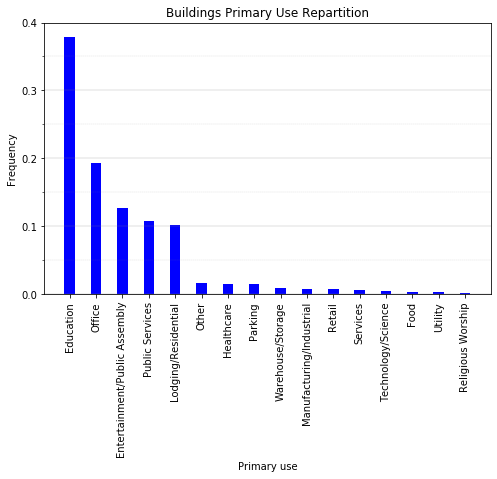
\includegraphics[scale=0.35]{../graphs/buildings_primary_use_repartition}
\caption{Buildings' primary use repartition}
\label{fig:buildings_primary_use_repartition}
\end{figure}

\begin{figure}[H]
\centering
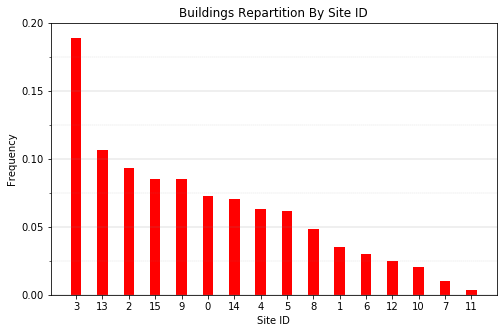
\includegraphics[scale=0.35]{../graphs/buildings_repartition_by_site_id}
\caption{Buildings' repartition by site ID}
\label{fig:buildings_repartition_by_site_id}
\end{figure}

\begin{figure}[H]
\centering
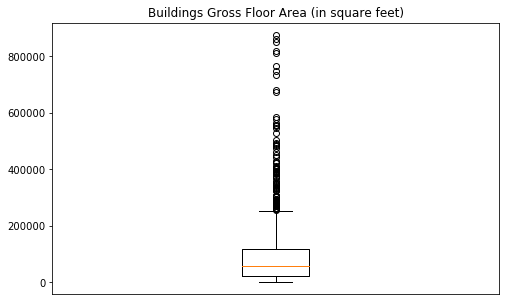
\includegraphics[scale=0.35]{../graphs/buildings_gross_floor_area}
\caption{Buildings' gross floor area variability}
\label{fig:buildings_gross_floor_area}
\end{figure}

Some statements can be made:

\begin{itemize}
\item It appears that for this study, the primary use of the buildings that have been taken into account is reparted around $16$ categories, not very well balanced, with a large majority of them (more than a third) dedicated to education. We can suppose that this feature has a great incidence over a building energy consumption, independently of its other characteristics: Indeed, a building dedicated to education works a very different way from another dedicated to religious worship, for example. Thus, it is quite probable that the prediction models we are going to build will present some kind of bias, due to the fact that they will be, in a great part, built thanks education buildings, and, so, will be consistent with this type of buildings, but probably not so with other types of buildings;
\item The buildings taken into account for this study are reparted around 16 different geographical sites, with their own specific weather conditions. As for previous conclusion, the observed repartition is not well balanced, thus, too, it is quite probable that the prediction models we are going to built will present some kind of bias, due to the fact that during the training they will be more exposed to some specific weather conditions;
\item Respectively to buildings gross floor area, we note approximately 7.32\% of outliers, element important to tackle, as it appears obvious that a building's gross floor area impacts its energy consumption.
\end{itemize}

During the exploration we performed of this tabular data file, we observed that the missing values are concentrated into $2$ columns, \textit{year\_built} and \textit{floor\_count}, and that these missing values represented a significant proportion of all registered values for these $2$ features (respectively 53.42\% and 75.50\%). Furthermore, we noted no strong correlation between each one of these $2$ features and the other ones (see Figures \ref{fig:buildings_year_built} and \ref{fig:buildings_floor_count}), which significates that these $2$ features contain proper information: This is a serious issue.

\begin{figure}[H]
\centering
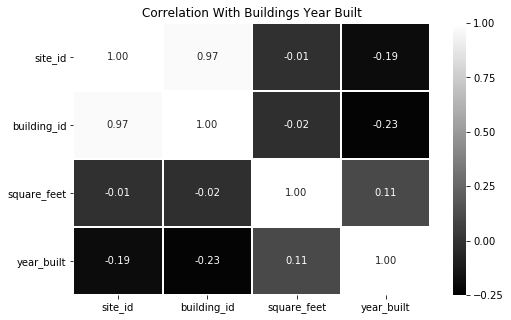
\includegraphics[scale=0.35]{../graphs/buildings_year_built}
\caption{Buildings' year built correlation matrix}
\label{fig:buildings_year_built}
\end{figure}

\begin{figure}[H]
\centering
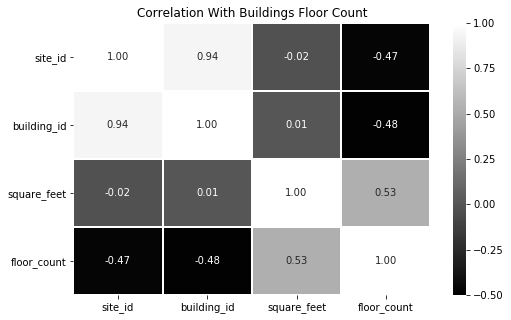
\includegraphics[scale=0.35]{../graphs/buildings_floor_count}
\caption{Buildings' floor count correlation matrix}
\label{fig:buildings_floor_count}
\end{figure}

\subsubsection{\textit{weather\_train.csv}}

The second tabular data file (see Table \ref{tab:weather}) contains, over the year $2016$, some weather's conditions registered on the various site IDs exploited during this study (see Figures \ref{fig:evolution_air_temperature_by_site_id}, \ref{fig:evolution_dew_temperature_by_site_id}, \ref{fig:evolution_wind_direction_by_site_id} and \ref{fig:evolution_wind_speed_by_site_id}).

\begin{figure}[H]
\centering
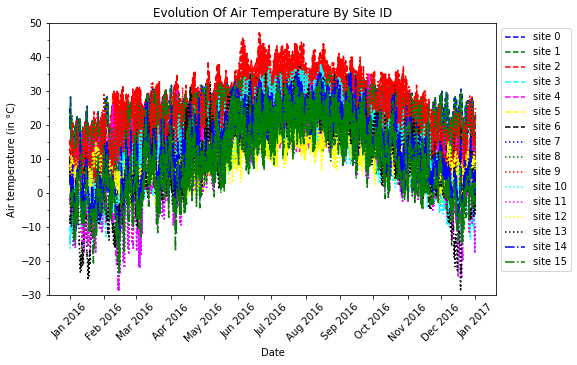
\includegraphics[scale=0.35]{../graphs/evolution_air_temperature_by_site_id}
\caption{Evolution of air temperature by site ID ($2016$)}
\label{fig:evolution_air_temperature_by_site_id}
\end{figure}

\begin{figure}[H]
\centering
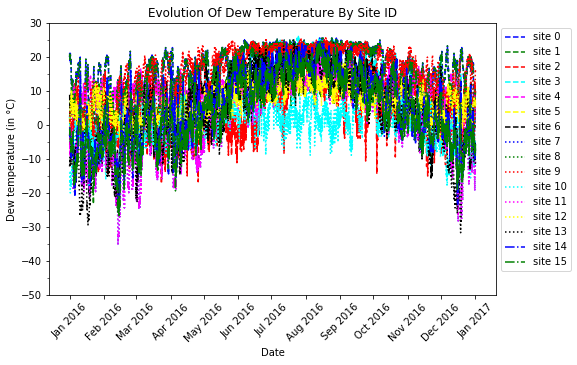
\includegraphics[scale=0.35]{../graphs/evolution_dew_temperature_by_site_id}
\caption{Evolution of dew temperature by site ID ($2016$)}
\label{fig:evolution_dew_temperature_by_site_id}
\end{figure}

\begin{figure}[H]
\centering
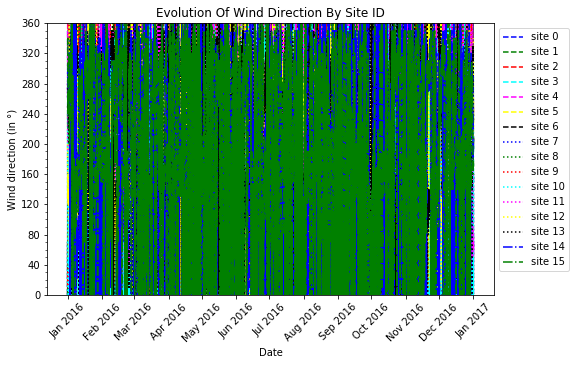
\includegraphics[scale=0.35]{../graphs/evolution_wind_direction_by_site_id}
\caption{Evolution of wind direction by site ID ($2016$)}
\label{fig:evolution_wind_direction_by_site_id}
\end{figure}

\begin{figure}[H]
\centering
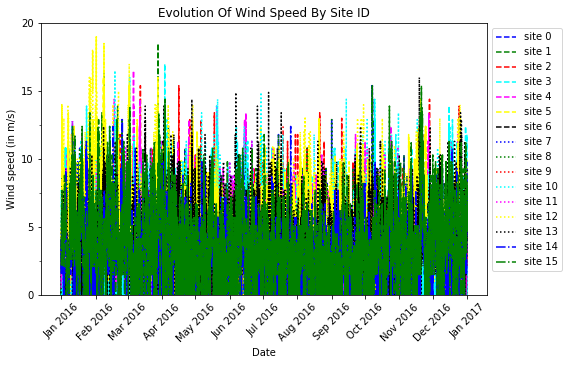
\includegraphics[scale=0.35]{../graphs/evolution_wind_speed_by_site_id}
\caption{Evolution of wind speed by site ID ($2016$)}
\label{fig:evolution_wind_speed_by_site_id}
\end{figure}

On this tabular data file, some conclusions can be stated:

\begin{itemize}
\item By site ID, evolution of air temperature, dew temperature, wind direction and wind speed covers un important spectrum of possibilities, nonetheless, for air temperature, for exemple, depending of the month of the year (and season), some common tendencies can be noted whatever the site ID considered: This will have an impact on the prediction models we will build, indeed, they will be trained only with data related to year $2016$, and they won't probably be able to catch year periodicity on the data and associated energy consumption (they won't probably be able to catch, too, certain epiphenomena, as Christmas and New Year holidays, element which provocs a discontinous and brutal change on energy consumption);
\item Features \textit{cloud\_coverage}, \textit{precip\_depth\_1\_hr}, and, to a lesser extent, \textit{sea\_level\_pressure}, count an import proportion of missing values (respectively 49.49\%, 35.98\% and 7.60\%), while this is not the case for the other features (less than 5\%). This is an important issue for these features (for \textit{cloud\_coverage}, e.g., we can reasonably assume that the impact on electricity consumption to light a building is not insignificant).
\end{itemize}

\subsubsection{\textit{train.csv}}

The third---and last---tabular data file (see Table \ref{tab:train}) contains, over the year $2016$, the various metered energy consumption registered.

First, we can consider Figure \ref{fig:energy_meter_repartition}.

\begin{figure}[H]
\centering
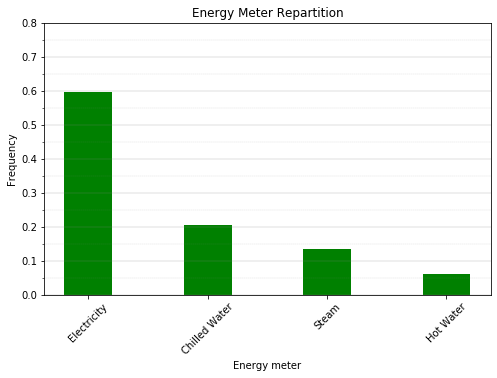
\includegraphics[scale=0.35]{../graphs/energy_meter_repartition}
\caption{Energy meter repartition ($2016$)}
\label{fig:energy_meter_repartition}
\end{figure}

As it can be observed, the energy meter repartition is not well balanced on the data set, this is not really an issue because we are going to build $4$ prediction models (one for each energy type), nevertheless, we can already suppose that the one we will build for electricity consumption prediction will probably be better than the one we will build for hot water consumption prediction (at least, we will benefit from more data to train the first one than we will benefit for training the second one).

Another interesting graph we can plot concerns the evolution of each energy type consumption over the year $2016$ (see Figures \ref{fig:evolution_electricity_consumption}, \ref{fig:evolution_chilled_water_consumption}, \ref{fig:evolution_steam_consumption} and \ref{fig:evolution_hot_water_consumption}).

\begin{figure}[H]
\centering
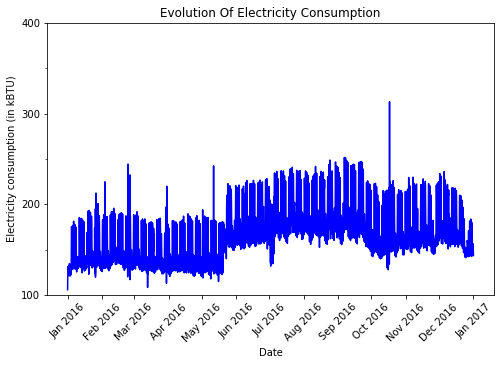
\includegraphics[scale=0.35]{../graphs/evolution_electricity_consumption}
\caption{Evolution of electricity consumption ($2016$)}
\label{fig:evolution_electricity_consumption}
\end{figure}

\begin{figure}[H]
\centering
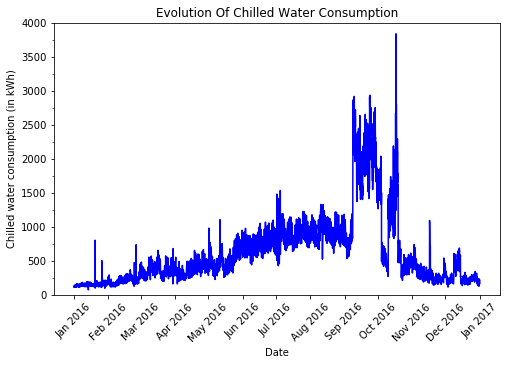
\includegraphics[scale=0.35]{../graphs/evolution_chilled_water_consumption}
\caption{Evolution of chilled water consumption ($2016$)}
\label{fig:evolution_chilled_water_consumption}
\end{figure}

\begin{figure}[H]
\centering
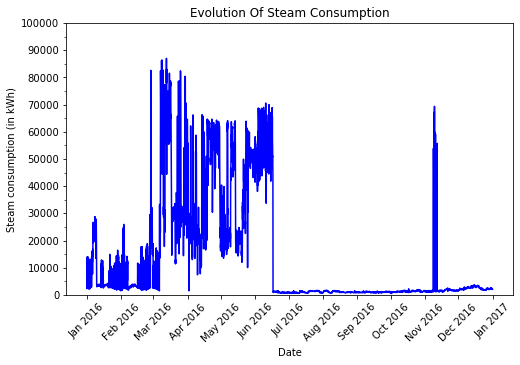
\includegraphics[scale=0.35]{../graphs/evolution_steam_consumption}
\caption{Evolution of steam consumption ($2016$)}
\label{fig:evolution_steam_consumption}
\end{figure}

\begin{figure}[H]
\centering
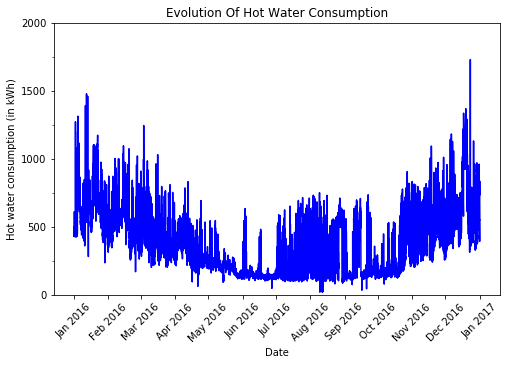
\includegraphics[scale=0.35]{../graphs/evolution_hot_water_consumption}
\caption{Evolution of hot water consumption ($2016$)}
\label{fig:evolution_hot_water_consumption}
\end{figure}

$3$ types of statements can be done respectively to these graphs:

\begin{itemize}
\item We can observe an high versatility on energy consumption data we benefit from, element that can be observed for each one of the $4$ energy types (we note, too, a proportion of outliers superior to 10\% for each one of them), we can thus already say that this will be a challenging point to handle for the prediction models we will build;
\item For this study, we benefit from one year of registered data, as we have previously noted when discussing weather conditions, this will have an impact on the prediction models we will build: Indeed, they will be trained only with data related to year $2016$, and they won't probably be able to catch year periodicity on the data and associated energy consumption (they won't probably be able to catch, too, certain epiphenomena, as Christmas and New Year holidays, element which provocs a discontinous and brutal change on energy consumption);
\item The graph exposing the evolution of steam consumption over the year used for this study seems quite "strange". Indeed, from june to december (with a very strange "Dirac epiphenomena" in November), it seems like if steam consumption meters have been inactive.
\end{itemize}

\subsection{Preprocessing}

We have now a better vision of the problem and the way we are going to tackle it:

\begin{enumerate}
\item The target variable is clearly identified, \textit{meter\_reading}, and is closely linked to variable \textit{meter}, which allows to indentify with which one of the $4$ energy types (electricity, chilled water, steam and hot water) it is related;
\item Before merging the $3$ tabular data files---\textit{building\_metadata.csv}, \textit{train.csv} and \textit{weather\_train.csv}---into one consistent data set, we need to perform independent operations:
\begin{itemize}
\item On tabular data files \textit{building\_metadata.csv} and \textit{weather\_train.csv}, we take the decision to drop features with too much missing values (features \textit{year\_built} and \textit{floor\_count} on tabular data file \textit{building\_metadata.csv}, and features \textit{cloud\_coverage}, \textit{precip\_depth\_1\_hr} and \textit{sea\_level\_pressure} on tabular data file \textit{weather\_train.csv});
\item On tabular data file \textit{weather\_train.csv}, we reconstruct missing values for features \textit{air\_temperature}, \textit{dew\_temperature}, \textit{wind\_direction} and \textit{wind\_speed}, replacing them by their previous value in the chronological process used to register data during the study;
\end{itemize}
\item After merging the $3$ tabular data files, $4$ steps need to be completed:
\begin{itemize}
\item Common outliers, independently from energy type, are removed (features \textit{square\_feet} and \textit{meter\_reading});
\item Cyclical features are transformed to take into account this aspect (features \textit{timestamp} and \textit{wind\_direction});
\item We handle \textit{primary\_use} categorical feature, making it a binary dummy variable;
\item We standardize continuous features (\textit{square\_feet}, \textit{air\_temperature}, \textit{dew\_temperature} and \textit{wind\_speed});
\end{itemize}
\item We terminate the preprocessing with the splitting of the data set into $4$ parts, each one of them corresponding to one particular energy type (electricity, chilled water, steam and hot water), and with removing outliers for meter reading registrations.
\end{enumerate}

This way, we obtain a consistent data set---to split, for each one of the $4$ energy types, between a training set (80\%) and a testing set (20\%) in a shuffled way---composed by:

\begin{itemize}
\item $9,868,987$ data points, $39$ feature variables and $1$ target variable for building electricity meter consumption forecasting model;
\item $2,922,250$ data points, $39$ feature variables and $1$ target variable for building chilled water meter consumption forecasting model;
\item $1,895,906$ data points, $39$ feature variables and $1$ target variable for building steam meter consumption forecasting model;
\item $791,788$ data points, $39$ feature variables and $1$ target variable for building hot water meter consumption forecasting model.
\end{itemize}

%% Problem Modeling %%

\section{Problem Modeling}

\subsection{General Methodology}

As it was precised in Subsection \ref{sub:problem_statement}, in this project, our main focus is to perform a "benchmarking" of $2$ current popular and very performant methods: Extreme Gradient Boosting (also known as XGBoost, see \cite{Chen_2016}) and Light Gradient Boosting Machine (also known as LightGBM, see \cite{Ke_2017}). For that, using Root Mean Squared Logarithmic Error (RMSLE) as quality metric to evaluate produced prediction models (see Subsection \ref{sub:quality_metric}) and a "naive" forecasting model (a forecasting prediction model which always predicts the mean value of all meter readings registered in each energy type data set), to appreciate the value provided by these $2$ methods, we are going to put them in action, and tune their hyperparameters as the hardware at our disposal (see Table \ref{tab:hardware}) allows us to do it.

Respectively to XGBoost, as precised in its documentation, we can note that:

\textit{"XGBoost is an optimized distributed gradient boosting library designed to be highly efficient, flexible and portable. It implements machine learning algorithms under the Gradient Boosting framework. XGBoost provides a parallel tree boosting (also known as GBDT, GBM) that solve many data science problems in a fast and accurate way."}\footnote{To obtain further information about Gradient Boosting, an interested reader can consult \cite{Friedman_2001}.}

In respect LightGBM, as written in its documentation, the following key points can be noted:

\textit{"LightGBM is a gradient boosting framework that uses tree based learning algorithms. It is designed to be distributed and efficient with the following advantages: Faster training speed and higher efficiency, lower memory usage, better accuracy, support of parallel and GPU learning, capable of handling large-scale data."}

Recently, both XGBoost and LightGBM have been widely-used in many winning solutions of machine learning competitions.

\subsection{Hyperparameters Tuning}

As discussed in Subsection above, the hardware at our disposal for this project constitutes a pain point, and, to a certain---and limited---point, we have only been able to perform hyperparameters' tuning with training data set dedicated to buildings' hot water meter energy consumption forecasting, the smallest of the $4$ ones for the problem to tackle.

Although, obviously, it's not the best solution to take, we have conserved the tuned hyperparameters we have obtained and used them for the $3$ other energy types: Indeed, same patterns can be observed in all energy types consumption, so, although it's not the best solution to take, it's not the worst either.

The "best" key hyperparameters we have obtained for XGBoost and LightGBM methods are expressed respectively in Table \ref{tab:xgboost_hyperparameters} and in Table \ref{tab:lightgbm_hyperparameters}.

\begin{table}[H]
\caption{XGBoost "best" key hyperparameters}
\centering
\begin{tabular}{ll}
\toprule
Number of gradient boosted trees & $77$ \\
Maximum tree depth for base learners & $9$ \\
Boosting learning rate & $0.4$ \\
Min loss reduction for tree's leaf node partition & $0.5$ \\
$L_1$ regularization term on weights & $5$ \\
$L_2$ regularization term on weights & $0.01$ \\
\bottomrule
\end{tabular}
\label{tab:xgboost_hyperparameters}
\end{table}

\begin{table}[H]
\caption{LightGBM "best" key hyperparameters}
\centering
\begin{tabular}{ll}
\toprule
Boosting type & DART \\
Number of boosted trees to fit & $100$ \\
Boosting learning rate & $1$ \\
Maximum tree depth for base learners & $5$ \\
$L_1$ regularization term on weights & $0.01$ \\
$L_2$ regularization term on weights & $0.01$ \\
\bottomrule
\end{tabular}
\label{tab:lightgbm_hyperparameters}
\end{table}

\subsection{Buildings' Electricity Meter Consumption Forecasting}

The results we obtained constructing buildings' electricity meter consumption forecasting models are summarized in Table \ref{tab:electricity_benchmarking}.

\begin{table}[H]
\caption{Buildings' electricity meter consumption forecasting models "benchmarking"}
\centering
\begin{tabular}{lll}
\toprule
Forecasting Model & RMSLE Score & \\
& Training Set & Testing Set \\
\midrule
"Naive" & $1.426128$ & $1.425909$ \\
XGBoost & $0.739577$ & $0.742597$ \\
LightGBM & $0.783755$ & $0.783860$ \\
\bottomrule
\end{tabular}
\label{tab:electricity_benchmarking}
\end{table}

As it can be observed, best scores, both on training and testing sets, are provided by XGBoost model.

An illustration of this benchmarking situation can be visualized on Figure \ref{fig:electricity_benchmarking_illustration}.

\begin{figure}[H]
\centering
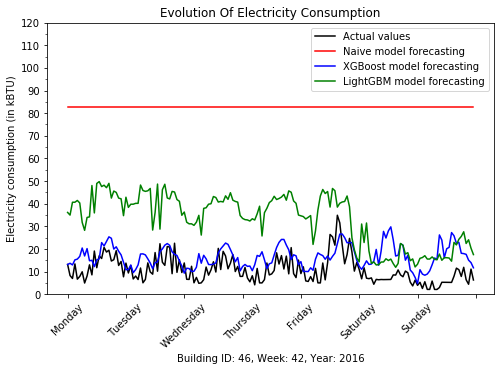
\includegraphics[scale=0.35]{../graphs/sample_electricity_consumption_comparison}
\caption{Buildings' electricity meter consumption forecasting models benchmarking illustration}
\label{fig:electricity_benchmarking_illustration}
\end{figure}

Finally, to explain XGBoost model predictions on testing set---data not used for building the model, so, data which allows to observe model's behaviour when confronted with "unknown" data, "real-life" data---, SHAP (SHapley Additive exPlanations) values have been mobilized, allowing us a better comprehension of the forecasting processing: This game theoretic approach is being increasingly used to explain the output of any machine learning model (see \cite{Lundberg_2017} and \cite{Lundberg_2020}).

An overview of which features are most important for the model is plotted on Figure \ref{fig:shap_values_summary_plot_electricity}, where the SHAP values of every feature for every sample are summarized.

\begin{figure}[H]
\centering
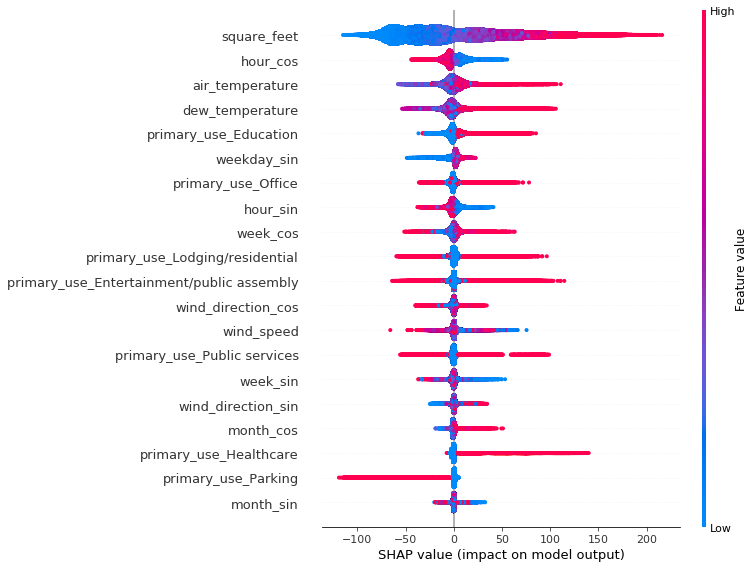
\includegraphics[scale=0.3]{../graphs/shap_values_summary_plot_electricity}
\caption{XGBoost model predictions on testing set explanation with SHAP values}
\label{fig:shap_values_summary_plot_electricity}
\end{figure}

The plot above sorts features by the sum of SHAP value magnitudes over all samples, and uses SHAP values to show the distribution of the impacts each feature has on the model output.

Here, we can observe what features drive the predictions on the testing set, and, thus, if we consider the "top 5" features, by order of importance, we have:

\begin{enumerate}
\item Surface of the building;
\item Hour's position in the day;
\item Air temperature;
\item Dew temperature;
\item Education as primary use.
\end{enumerate}

So, for example, analyzing the $2$ most important features, in accordance with what was intuitively expected, we can note that the highest the building's surface is, the more electricity consumption will be, and that being during labour hours, electricity consumption increases. It is equally interesting, too, to observe that air temperature and dew temperature have an important impact with the predictions of our model. Furthermore, if building's primary use belongs to education, office, residence, public assembly, public services, healthcare and parking, this aspect seems to be very discriminating for electricity consumption forecasting model's processing.

\subsection{Buildings' Chilled Water Meter Consumption Forecasting}

The results we obtained constructing buildings' chilled water meter consumption forecasting models are summarized in Table \ref{tab:chilled_water_benchmarking}.

\begin{table}[H]
\caption{Buildings' chilled water meter consumption forecasting models "benchmarking"}
\centering
\begin{tabular}{lll}
\toprule
Forecasting Model & RMSLE Score & \\
& Training Set & Testing Set \\
\midrule
"Naive" & $1.894896$ & $1.894816$ \\
XGBoost & $0.919122$ & $0.927294$ \\
LightGBM & $1.216306$ & $1.217206$ \\
\bottomrule
\end{tabular}
\label{tab:chilled_water_benchmarking}
\end{table}

As it can be observed, best scores, both on training and testing sets, are provided by XGBoost model.

An illustration of this benchmarking situation can be visualized on Figure \ref{fig:chilled_water_benchmarking_illustration}.

\begin{figure}[H]
\centering
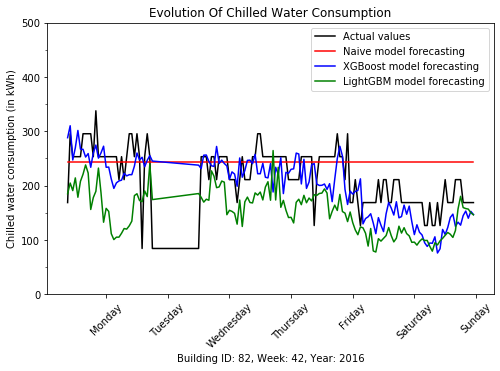
\includegraphics[scale=0.35]{../graphs/sample_chilled_water_consumption_comparison}
\caption{Buildings' chilled water meter consumption forecasting models benchmarking illustration}
\label{fig:chilled_water_benchmarking_illustration}
\end{figure}

As it has been done in previous Subsection, exploiting SHAP values, we are now going to explain XGBoost model predictions on testing set.

An overview of which features are most important for the model is plotted on Figure \ref{fig:shap_values_summary_plot_chilled_water}, where the SHAP values of every feature for every sample are summarized.

\begin{figure}[H]
\centering
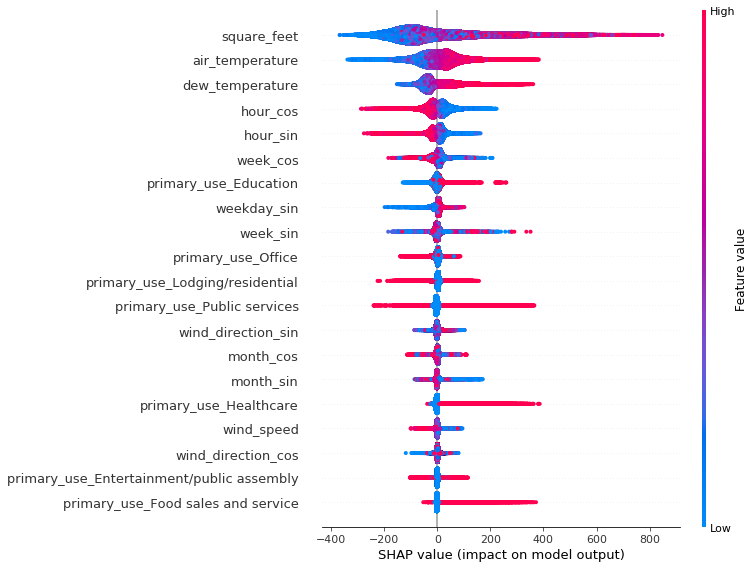
\includegraphics[scale=0.3]{../graphs/shap_values_summary_plot_chilled_water}
\caption{XGBoost model predictions on testing set explanation with SHAP values}
\label{fig:shap_values_summary_plot_chilled_water}
\end{figure}

In this graph, we can observe what features drive the predictions on the testing set, and, thus, if we consider the "top 4" features, by order of importance, we have:

\begin{enumerate}
\item Surface of the building;
\item Air temperature;
\item Dew temperature;
\item hour's position in the day.
\end{enumerate}

So, as previously, for example, analyzing the $2$ most important features, in accordance with what was intuitively expected, we can note that the highest the building's surface is, the more chilled water consumption will be, and, the hotest the air temperature is, the more chilled water consumption will be. It is equally interesting, too, to observe that dew temperature is the third most important feature for the model we have built, and that afternoons use to be moments in the day when chilled water consumption is high. Furthermore, if building's primary use belongs to public services, healthcare and food sales and service, this aspect seems to be very discriminating for chilled water consumption forecasting model's processing.

\subsection{Buildings' Steam Meter Consumption Forecasting}

The results we obtained constructing buildings' steam meter consumption forecasting models are summarized in Table \ref{tab:steam_benchmarking}.

\begin{table}[H]
\caption{Buildings' steam meter consumption forecasting models "benchmarking"}
\centering
\begin{tabular}{lll}
\toprule
Forecasting Model & RMSLE Score & \\
& Training Set & Testing Set \\
\midrule
"Naive" & $1.760635$ & $1.759955$ \\
XGBoost & $0.818102$ & $0.831114$ \\
LightGBM & $1.026755$ & $1.030987$ \\
\bottomrule
\end{tabular}
\label{tab:steam_benchmarking}
\end{table}

As it can be observed, best scores, both on training and testing sets, are provided by XGBoost model.

An illustration of this benchmarking situation can be visualized on Figure \ref{fig:steam_benchmarking_illustration}.

\begin{figure}[H]
\centering
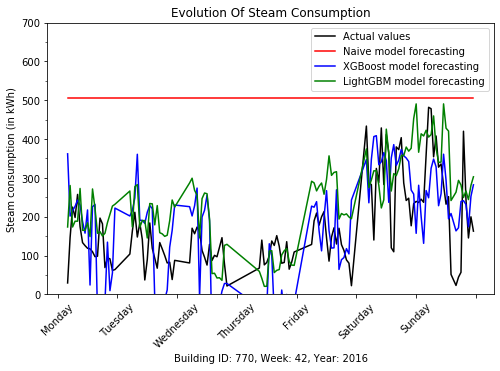
\includegraphics[scale=0.35]{../graphs/sample_steam_consumption_comparison}
\caption{Buildings' steam meter consumption forecasting models benchmarking illustration}
\label{fig:steam_benchmarking_illustration}
\end{figure}

As it has been done in previous Subsections, exploiting SHAP values, we are now going to explain XGBoost model predictions on testing set.

An overview of which features are most important for the model is plotted on Figure \ref{fig:shap_values_summary_plot_steam}, where the SHAP values of every feature for every sample are summarized.

\begin{figure}[H]
\centering
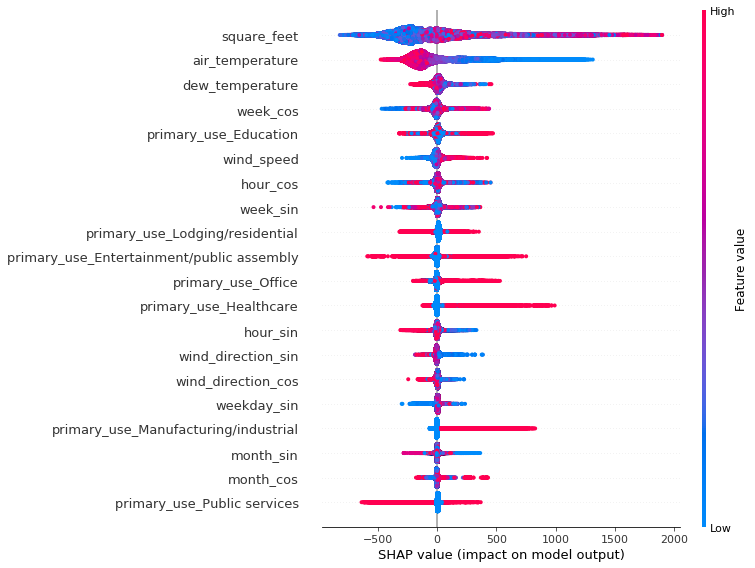
\includegraphics[scale=0.3]{../graphs/shap_values_summary_plot_steam}
\caption{XGBoost model predictions on testing set explanation with SHAP values}
\label{fig:shap_values_summary_plot_steam}
\end{figure}

In this graph, we can observe what features drive the predictions on the testing set, and, thus, if we consider the "top 5" features, by order of importance, we have:

\begin{enumerate}
\item Surface of the building;
\item Air temperature;
\item Dew temperature;
\item Week's position in the year;
\item Education as primary use.
\end{enumerate}

So, for example, analyzing the $2$ most important features, in accordance with what was intuitively expected, we can note that the highest the building's surface is, the more steam consumption will be, and, the hotest the air temperature is, the less steam consumption will be. It is equally interesting, too, to observe that dew temperature is the third most important feature for the model we have built. Furthermore, if building's primary use belongs to public assembly, healthcare, industry and public services, this aspect seems to be very discriminating for steam consumption forecasting model's processing.

\subsection{Buildings' Hot Water Meter Consumption Forecasting}

The results we obtained constructing buildings' hot water meter consumption forecasting models are summarized in Table \ref{tab:hot_water_benchmarking}.

\begin{table}[H]
\caption{Buildings' hot water meter consumption forecasting models "benchmarking"}
\centering
\begin{tabular}{lll}
\toprule
Forecasting Model & RMSLE Score & \\
& Training Set & Testing Set \\
\midrule
"Naive" & $1.979692$ & $1.982237$ \\
XGBoost & $0.850988$ & $0.881483$ \\
LightGBM & $1.030566$ & $1.035321$ \\
\bottomrule
\end{tabular}
\label{tab:hot_water_benchmarking}
\end{table}

As it can be observed, best scores, both on training and testing sets, are provided by XGBoost model.

An illustration of this benchmarking situation can be visualized on Figure \ref{fig:hot_water_benchmarking_illustration}.

\begin{figure}[H]
\centering
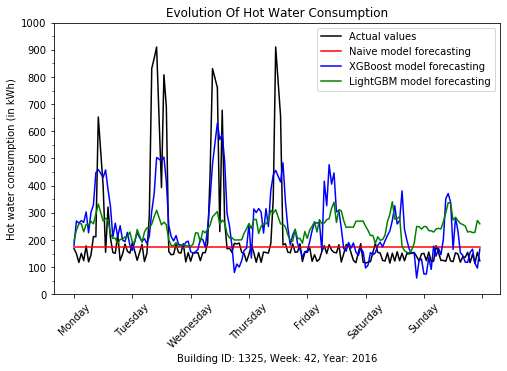
\includegraphics[scale=0.35]{../graphs/sample_hot_water_consumption_comparison}
\caption{Buildings' hot water meter consumption forecasting models benchmarking illustration}
\label{fig:hot_water_benchmarking_illustration}
\end{figure}

As it has been done in previous Subsections, exploiting SHAP values, we are now going to explain XGBoost model predictions on testing set.

An overview of which features are most important for the model is plotted on Figure \ref{fig:shap_values_summary_plot_hot_water}, where the SHAP values of every feature for every sample are summarized.

\begin{figure}[H]
\centering
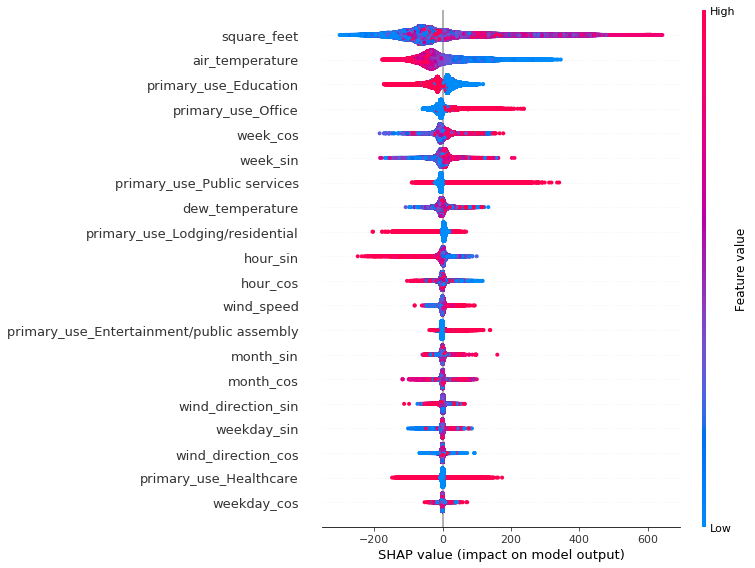
\includegraphics[scale=0.3]{../graphs/shap_values_summary_plot_hot_water}
\caption{XGBoost model predictions on testing set explanation with SHAP values}
\label{fig:shap_values_summary_plot_hot_water}
\end{figure}

In this graph, we can observe what features drive the predictions on the testing set, and, thus, if we consider the "top 5" features, by order of importance, we have:

\begin{enumerate}
\item Surface of the building;
\item Air temperature;
\item Education as primary use;
\item Office as primary use;
\item Week's position in the year.
\end{enumerate}

So, for example, analyzing the $2$ most important features, in accordance with what was intuitively expected, we can note that the highest the building's surface is, the more hot water consumption will be, and, the hotest the air temperature is, the less hot water consumption will be. It is interesting to note, too, that building's primary use (especially education, office, public services and healthcare) seems to have disruptive impact for hot water consumption forecasting model's processing.

%% Proposed Solution %%

\section{Proposed Solution}

To conclude this report and our analysis on the challenge to tackle, based on the various statements and conclusions that have been established, we are led to propose XGBoost models to forecast each one of the buildings' $4$ energy types metered consumption (electricity, chilled water, steam and hot water). Indeed, it's with these models---despite the limited hyperparameters tuning the hardware has allowed us to perform---the best scores have been reached.

Nevertheless, some indications can be provided to go further this work and deepen it:

\begin{itemize}
\item Firstly, a more complete work can be performed about the data put at disposal, principally about missing data and ways to explore to try te reconstruct it. For example, respectively to the data linked to weather conditions, trying to figure out the exact localizations of the $16$ site IDs mobilized for this study, it's probably possible to gather the needed information to fill missing values, or at least some of them.
\item Secondly, with less limited hardware, a consistent work about hyperparameters tuning---for both XGBoost and LightGBM models---could be realized. Here, we have operated a randomized search on key hyperparameters of both XGBoost and LightGBM, but we have been very limited in our action. An interesting perspective to explore---and a smarter way to proceed---is to combine randomized search and grid search: In a first step, randomized search can be used with a large hyperparameters grid, then, in a second step, exploiting the results that have been obtained, a focused hyperparameters grid around the best performing hyperparameters values can be established, and, after that, in a third step, a grid search can be run on this reduced hyperparameters grid, process that can be reapeted (until maximum computational/time budget is exceeded). Bayesian hyperparameters optimization could equally constitute an interesting way to follow (see, e.g., \cite{Bergstra_2013}).
\item Thirdly, and lastly, more complex architectures for the forecasting process can be tried to reach better scores (e.g., using a voting regressor, or decomposing data domain used for training).
\end{itemize}


%%%%%%%%%%%%%%%%%%%%%%%%%%%%%%%%%%%%%%%%%%%%%%%%%
%                BIBLIOGRAPHY                   %
%%%%%%%%%%%%%%%%%%%%%%%%%%%%%%%%%%%%%%%%%%%%%%%%%

\begin{normalsize}
\bibliography{references}
\end{normalsize}


%%%%%%%%%%%%%%%%%%%%%%%%%%%%%%%%%%%%%%%%%%%%%%%%%
%                     END                       %
%%%%%%%%%%%%%%%%%%%%%%%%%%%%%%%%%%%%%%%%%%%%%%%%%

\end{document}